\section{期望误差}
\label{sec:dcomp-expectation}

比较分布往往是为了一个具体目的：用$Q$代替$P$计算某个平均$\mathbb{E}_{P}[g]$，误差有多大？前面几节已经分别得到有界函数、Lipschitz函数与RKHS函数的期望差表示。把这些结果放在一起，问题就变成：给定的$g$属于哪一类，范数是多少，该用哪个比较量。无界的$g$不属于这些类中的某几个，需要另外控制尾部；KL散度不是积分概率度量，要借助指数矩才能控制期望。

\subsection{函数范围内的误差}
\label{sec:dcomp-function-bounds}

把式~\eqref{eq:dcomp-tv-osc}、式~\eqref{eq:dcomp-kr}与式~\eqref{eq:dcomp-mmd-def}中的函数类按范数缩放，就得到三个上界。

\begin{theorem}[三类函数的期望差]
\label{thm:dcomp-three-bounds}
设$P,Q$是同一空间上的概率分布。
\begin{enumerate}
 \item 若$g$可测且有界，则期望差的绝对值不超过$\operatorname{osc}(g)\,d_{\mathrm{TV}}(P,Q)$。
 \item 若空间是Polish空间，$P,Q\in\mathcal{P}_1$，$g$是Lipschitz函数，常数为$\operatorname{Lip}(g)$，则
 \begin{equation}
  \bigl\lvert\mathbb{E}_{P}[g]-\mathbb{E}_{Q}[g]\bigr\rvert\leq\operatorname{Lip}(g)\,W_1(P,Q) .
  \label{eq:dcomp-lip-bound}
 \end{equation}
 \item 若$k$满足定理~\ref{thm:dcomp-kernel-mean}的条件，$P,Q$满足式~\eqref{eq:dcomp-kernel-moment}，$g\in\mathcal{H}$，则
 \begin{equation}
  \bigl\lvert\mathbb{E}_{P}[g]-\mathbb{E}_{Q}[g]\bigr\rvert\leq\lVert g\rVert_{\mathcal{H}}\operatorname{MMD}_k(P,Q) .
  \label{eq:dcomp-rkhs-bound}
 \end{equation}
\end{enumerate}
\end{theorem}

\begin{proof}
第一条即式~\eqref{eq:dcomp-tv-osc}。第二条：$\operatorname{Lip}(g)=0$时$g$为常数，两边为零；否则$g/\operatorname{Lip}(g)$是1-Lipschitz函数，由式~\eqref{eq:dcomp-kr}得结论，$g$在$P,Q$下可积已在第~\ref{sec:dcomp-kr}节说明。第三条：$g=0$时两边为零；否则$g/\lVert g\rVert_{\mathcal{H}}$在单位球中，由式~\eqref{eq:dcomp-mmd-def}得结论。
\end{proof}

定理的三条要求不同的东西，选择哪一条取决于$g$的性质。示性函数$\mathbf{1}_{A}$有界，但有跳跃，不是Lipschitz函数，也不在高斯核的RKHS中（该空间中的函数都连续），只能用总变差。$g(x)=x$是1-Lipschitz函数，但无界；高斯核有界，由定理~\ref{thm:dcomp-kernel-mean}证明中的估计，$\lvert g(x)\rvert$不超过$\lVert g\rVert_{\mathcal{H}}\sqrt{k(x,x)}$，而高斯核的$k(x,x)=1$，所以它的RKHS只含有界函数，所以只能用$W_1$。光滑、有界的函数三条都可以用，这时要比较哪个上界更小。

\paragraph{同一个函数的三个上界}
取$P=\delta_0$，$Q=\delta_h$，$g(x)=\exp(-x^{2}/2)$，它是$\sigma=1$高斯核的截面$k(0,\cdot)$。由式~\eqref{eq:dcomp-reproducing}，$\lVert g\rVert_{\mathcal{H}}=\sqrt{k(0,0)}=1$；它的振幅为$1$；导数$-x\mathrm{e}^{-x^{2}/2}$的绝对值在$x=\pm1$处最大，Lipschitz常数是$\mathrm{e}^{-1/2}\approx0.6065$。真实的误差和三个上界分别是
\[
 1-\mathrm{e}^{-h^{2}/2},\qquad 1,\qquad\mathrm{e}^{-1/2}h,\qquad\sqrt{2-2\mathrm{e}^{-h^{2}/2}} .
\]
$h=0.5$时，真实误差约为$0.1175$，$W_1$上界约为$0.3033$，MMD上界约为$0.4848$，总变差上界是$1$。图~\ref{fig:dcomp-three-bounds}显示，小平移时$W_1$的界最紧，大平移时总变差的界最紧（误差本来就不会超过振幅），MMD的界在两者之间过渡。没有哪一个比较量对所有情形都最好。

\begin{BookInlineFigure}
 \centering
 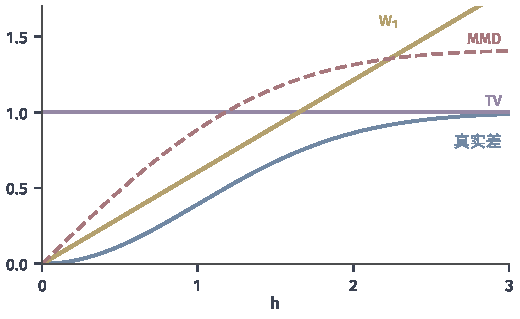
\includegraphics[width=88mm]{figures/07-probability/04-distribution-analysis/matplotlib/dcomp-three-bounds/figure.pdf}
 \caption{$P=\delta_0$，$Q=\delta_h$，$g(x)=\mathrm{e}^{-x^{2}/2}$时的期望误差。蓝线是真实误差$1-\mathrm{e}^{-h^{2}/2}$；紫线是总变差上界$\operatorname{osc}(g)\,d_{\mathrm{TV}}=1$，黄线是$W_1$上界$\mathrm{e}^{-1/2}h$，红色虚线是MMD上界$\sqrt{2-2\mathrm{e}^{-h^{2}/2}}$。}
 \label{fig:dcomp-three-bounds}
\end{BookInlineFigure}

\subsection{无界函数的尾部控制}
\label{sec:dcomp-tail}

许多需要计算的平均来自无界函数：均值、方差、多项式损失。分布在总变差或MMD意义下接近，只说明大部分质量摆放得差不多；极少的质量若落在很远的地方，无界函数会把它放大。下面先给出一个把问题拆开的不等式，再看反例。

\begin{lemma}[截断分解]
\label{lem:dcomp-truncation}
设$g$在$P,Q$下可积，$r>0$。记$g_r$为$g$在水平$r$处的截断，即把大于$r$的值改为$r$，小于$-r$的值改为$-r$。则
\begin{equation}
 \begin{aligned}
 \bigl\lvert\mathbb{E}_{P}[g]-\mathbb{E}_{Q}[g]\bigr\rvert&\leq\bigl\lvert\mathbb{E}_{P}[g_r]-\mathbb{E}_{Q}[g_r]\bigr\rvert\\
 &\quad+\mathbb{E}_{P}\bigl[\lvert g\rvert\mathbf{1}_{\{\lvert g\rvert>r\}}\bigr]+\mathbb{E}_{Q}\bigl[\lvert g\rvert\mathbf{1}_{\{\lvert g\rvert>r\}}\bigr] .
 \end{aligned}
 \label{eq:dcomp-truncation}
\end{equation}
\end{lemma}

\begin{proof}
$g-g_r$只在$\{\lvert g\rvert>r\}$上非零，那里$g-g_r$的绝对值是$\lvert g\rvert-r$，不超过$\lvert g\rvert$，所以
\[
 \bigl\lvert\mathbb{E}_{P}[g-g_r]\bigr\rvert\leq\mathbb{E}_{P}\bigl[\lvert g\rvert\mathbf{1}_{\{\lvert g\rvert>r\}}\bigr],
\]
对$Q$同理。把$g=g_r+(g-g_r)$代入期望差，用三角不等式即得。
\end{proof}

右边第一项是有界函数的期望差，可用前面的比较量控制，例如不超过$2r\,d_{\mathrm{TV}}(P,Q)$；若$g$是Lipschitz函数，$g_r$也是，并且常数不变，可以用$W_1$。后两项是两个分布各自的尾部，比较量对它们无能为力，必须由矩条件单独控制。对一列分布，需要的就是尾部的一致小。

\begin{theorem}[一致可积时期望收敛]
\label{thm:dcomp-ui-convergence}
设$d_{\mathrm{TV}}(P_n,P)\to0$，$g$在每个$P_n$与$P$下可积，并且
\begin{equation}
 \lim_{r\to\infty}\sup_{n}\mathbb{E}_{P_n}\bigl[\lvert g\rvert\mathbf{1}_{\{\lvert g\rvert>r\}}\bigr]=0 .
 \label{eq:dcomp-ui}
\end{equation}
则$\mathbb{E}_{P_n}[g]\to\mathbb{E}_{P}[g]$。
\end{theorem}

\begin{proof}
任给$\varepsilon>0$。由式~\eqref{eq:dcomp-ui}与$\mathbb{E}_{P}\lvert g\rvert<\infty$，可以取$r$，使式~\eqref{eq:dcomp-truncation}的两个尾部项对每个$P_n$与$P$都小于$\varepsilon$。由式~\eqref{eq:dcomp-truncation}与$\operatorname{osc}(g_r)\leq2r$，
\[
 \bigl\lvert\mathbb{E}_{P_n}[g]-\mathbb{E}_{P}[g]\bigr\rvert\leq2r\,d_{\mathrm{TV}}(P_n,P)+2\varepsilon .
\]
固定$r$令$n\to\infty$，上极限不超过$2\varepsilon$；$\varepsilon$任意，结论成立。
\end{proof}

条件~\eqref{eq:dcomp-ui}正是第~\ref{chap:random-variable-convergence}章的一致可积。多项式增长的函数可以用高一点的矩保证它。设$\lvert g(x)\rvert\leq C(1+\lvert x\rvert^{k})$，并且对某个$\delta>0$，各$P_n$的$k+\delta$阶绝对矩一致地不超过$M$。记$q=1+\delta/k$。在$\{\lvert g\rvert>r\}$上，$\lvert g\rvert\leq\lvert g\rvert^{q}/r^{q-1}$，又由$(a+b)^{q}\leq2^{q-1}(a^{q}+b^{q})$，
\[
 \mathbb{E}_{P_n}\bigl[\lvert g\rvert\mathbf{1}_{\{\lvert g\rvert>r\}}\bigr]\leq\frac{\mathbb{E}_{P_n}\lvert g\rvert^{q}}{r^{q-1}}\leq\frac{C^{q}2^{q-1}(1+M)}{r^{\delta/k}},
\]
关于$n$一致地趋于零。只有$k$阶矩有界是不够的，下面的例子说明这一点。

\paragraph{远处的小质量}
令$P_n=(1-\tfrac1n)\delta_0+\tfrac1n\delta_n$，与$\delta_0$比较。总变差是$1/n$，高斯核MMD约为$\sqrt2/n$，都趋于零。每个$P_n$只有两个支撑点，各阶矩都有限。可是均值与二阶矩是
\[
 \mathbb{E}_{P_n}[X]=\frac1n\cdot n=1,\qquad\mathbb{E}_{P_n}[X^{2}]=\frac1n\cdot n^{2}=n,
\]
不收敛到$\delta_0$下的$0$。尾部条件~\eqref{eq:dcomp-ui}对$g(x)=x$不成立：$n>r$时$\mathbb{E}_{P_n}[X\mathbf{1}_{\{X>r\}}]=1$。逐个分布的矩有限，不能代替一致的尾部控制。

$W_1$能看见这一份远处的质量：把$1/n$的质量从$n$搬回$0$，成本是$1$，所以$W_1(P_n,\delta_0)=1$，与均值的差一致，这正是式~\eqref{eq:dcomp-lip-bound}对$g(x)=x$的含义。但$W_1$也有看不见的东西。令
\[
 R_n=(1-n^{-2})\delta_0+n^{-2}\delta_n .
\]
把$n^{-2}$的质量搬动距离$n$，一阶与二阶的搬运成本分别给出
\[
 W_1(R_n,\delta_0)=\frac1n\to0,\qquad W_2(R_n,\delta_0)=\bigl(n^{-2}\cdot n^{2}\bigr)^{1/2}=1 ,
\]
而$R_n$的二阶矩恒为$1$，不趋于零。图~\ref{fig:dcomp-far-mass}画出这两族分布。控制$k$阶增长的函数，要用$k$阶的比较量或额外的一致可积条件。

\begin{BookInlineFigure}
 \centering
 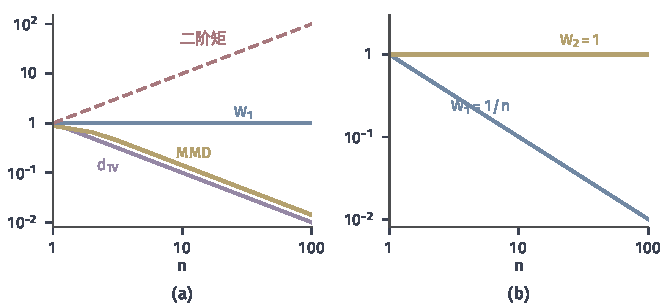
\includegraphics[width=112mm]{figures/07-probability/04-distribution-analysis/matplotlib/dcomp-far-mass/figure.pdf}
 \caption{远处的小质量，与$\delta_0$比较，双对数坐标。(a)$P_n=(1-\tfrac1n)\delta_0+\tfrac1n\delta_n$：$d_{\mathrm{TV}}=1/n$（紫），$\sigma=1$高斯核MMD（黄），$W_1=1$（蓝），二阶矩$n$（红色虚线）。(b)$R_n=(1-n^{-2})\delta_0+n^{-2}\delta_n$：$W_1=1/n$（蓝），$W_2=1$（黄）。}
 \label{fig:dcomp-far-mass}
\end{BookInlineFigure}

\subsection{KL与指数矩}
\label{sec:dcomp-kl-exp}

KL散度没有写成积分概率度量的形式，它能控制期望吗？先看有界函数：第~\ref{sec:dcomp-pinsker}节将证明KL散度控制总变差，于是它也控制有界函数的期望差。对无界函数，KL散度单独不够，还需要参考分布$Q$下的指数矩。关键工具是把$Q$按$\mathrm{e}^{g}$重新加权。

设$g$可测，$Z=\mathbb{E}_{Q}[\mathrm{e}^{g}]<\infty$。定义新的分布$Q_g$，
\begin{equation}
 \frac{\mathrm{d}Q_g}{\mathrm{d}Q}=\frac{\mathrm{e}^{g}}{Z} .
 \label{eq:dcomp-tilt}
\end{equation}
它把$Q$的质量向$g$大的地方倾斜，称为\term{指数倾斜}（exponential tilting）。密度$\mathrm{e}^{g}/Z$处处为正，所以$Q$与$Q_g$互相绝对连续。

\begin{lemma}[KL与对数矩母函数]
\label{lem:dcomp-dv}
设$D_{\mathrm{KL}}(P\Vert Q)<\infty$，$\mathbb{E}_{Q}[\mathrm{e}^{g}]<\infty$，$\mathbb{E}_{P}\lvert g\rvert<\infty$。则
\begin{equation}
 \mathbb{E}_{P}[g]\leq D_{\mathrm{KL}}(P\Vert Q)+\ln\mathbb{E}_{Q}\bigl[\mathrm{e}^{g}\bigr] .
 \label{eq:dcomp-dv}
\end{equation}
\end{lemma}

\begin{proof}
$P\ll Q$，$Q\ll Q_g$，所以$P\ll Q_g$，并且由密度的链式法则与式~\eqref{eq:dcomp-tilt}，
\[
 \ln\frac{\mathrm{d}P}{\mathrm{d}Q_g}=\ln\frac{\mathrm{d}P}{\mathrm{d}Q}-g+\ln Z .
\]
$D_{\mathrm{KL}}(P\Vert Q)$有限且对数比的负部可积，所以$\ln(\mathrm{d}P/\mathrm{d}Q)$在$P$下可积；$g$也可积。对上式在$P$下逐项取期望，并用Gibbs不等式，
\[
 0\leq D_{\mathrm{KL}}(P\Vert Q_g)=D_{\mathrm{KL}}(P\Vert Q)-\mathbb{E}_{P}[g]+\ln Z .
\]
移项即得。
\end{proof}

不等式~\eqref{eq:dcomp-dv}只是把KL的非负性用在倾斜后的参考分布上。它的含义是：$P$相对$Q$偏离不大时，$g$在$P$下的平均不会远超“$Q$下的指数平均”。为了得到期望差，对$g$减去它在$Q$下的均值并乘以参数$\lambda$。

\begin{theorem}[KL控制的期望差]
\label{thm:dcomp-kl-expectation}
设$D_{\mathrm{KL}}(P\Vert Q)<\infty$，$g$在$P,Q$下可积，记
\begin{equation}
 \Lambda(\lambda)=\ln\mathbb{E}_{Q}\Bigl[\exp\bigl(\lambda(g-\mathbb{E}_{Q}[g])\bigr)\Bigr] .
 \label{eq:dcomp-centered-cgf}
\end{equation}
则对每个使$\Lambda(\lambda)$有限的$\lambda>0$，
\begin{equation}
 \begin{gathered}
 \mathbb{E}_{P}[g]-\mathbb{E}_{Q}[g]\leq\frac{D_{\mathrm{KL}}(P\Vert Q)+\Lambda(\lambda)}{\lambda},\\
 \mathbb{E}_{Q}[g]-\mathbb{E}_{P}[g]\leq\frac{D_{\mathrm{KL}}(P\Vert Q)+\Lambda(-\lambda)}{\lambda} .
 \end{gathered}
 \label{eq:dcomp-kl-two-sides}
\end{equation}
特别地，若对一切实数$\lambda$有$\Lambda(\lambda)\leq\lambda^{2}s^{2}/2$，则
\begin{equation}
 \bigl\lvert\mathbb{E}_{P}[g]-\mathbb{E}_{Q}[g]\bigr\rvert\leq\sqrt{2s^{2}D_{\mathrm{KL}}(P\Vert Q)} .
 \label{eq:dcomp-kl-subgaussian}
\end{equation}
\end{theorem}

\begin{proof}
把引理~\ref{lem:dcomp-dv}用于$\lambda(g-\mathbb{E}_{Q}[g])$，它在$P$下可积，在$Q$下的指数矩是$\mathrm{e}^{\Lambda(\lambda)}$：
\[
 \lambda\bigl(\mathbb{E}_{P}[g]-\mathbb{E}_{Q}[g]\bigr)\leq D_{\mathrm{KL}}(P\Vert Q)+\Lambda(\lambda) .
\]
除以$\lambda>0$得第一式。把同样的推理用于$-g$，它的中心化对数矩母函数是$\Lambda(-\lambda)$，得第二式。在次高斯条件下，两式右端都不超过$D/\lambda+\lambda s^{2}/2$（记$D=D_{\mathrm{KL}}(P\Vert Q)$）。$D>0$时取$\lambda=\sqrt{2D}/s$使它最小，最小值为$\sqrt{2s^{2}D}$；$D=0$时$P=Q$，两边都是零。
\end{proof}

\paragraph{高斯平移}
取$Q=\mathcal{N}(0,1)$与$g(x)=x$。中心化对数矩母函数是$\Lambda(\lambda)=\lambda^{2}/2$，次高斯条件以$s=1$成立。倾斜后的$Q_g$在$g=\lambda x$时是$\mathcal{N}(\lambda,1)$：$\mathrm{e}^{\lambda x}$乘以标准高斯密度，配方后正是均值为$\lambda$的高斯密度。再取$P$为均值$m$、方差$1$的高斯分布，由式~\eqref{eq:dcomp-kl-gauss}，KL散度是$m^{2}/2$，式~\eqref{eq:dcomp-kl-subgaussian}给出
\[
 \lvert\mathbb{E}_{P}[X]-\mathbb{E}_{Q}[X]\rvert\leq\sqrt{2\cdot m^{2}/2}=\lvert m\rvert ,
\]
等号成立，上界不能改进。若$P=\mathcal{N}(m,s'^{2})$，均值差仍是$m$，而KL散度多了方差失配的部分，上界变松；$m=1$时，$s'=\tfrac12$与$s'=2$的上界分别约为$1.279$与$1.617$。图~\ref{fig:dcomp-kl-tilt}画出倾斜后的分布与这些上界。

\begin{BookInlineFigure}
 \centering
 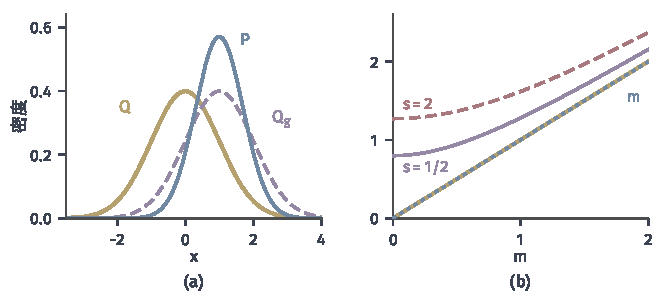
\includegraphics[width=112mm]{figures/07-probability/04-distribution-analysis/matplotlib/dcomp-kl-tilt/figure.pdf}
 \caption{KL散度与指数矩，$Q=\mathcal{N}(0,1)$，$g(x)=x$。(a)$Q$（黄），按$\mathrm{e}^{x}$倾斜后的$Q_g=\mathcal{N}(1,1)$（紫色虚线），以及$P=\mathcal{N}(1,0.7^{2})$（蓝）。(b)$P=\mathcal{N}(m,s'^{2})$时的真实均值差$m$（蓝色点线）与上界$\sqrt{2D_{\mathrm{KL}}(P\Vert Q)}$：$s'=1$（黄，与真实值重合），$s'=\tfrac12$（紫），$s'=2$（红色虚线）。}
 \label{fig:dcomp-kl-tilt}
\end{BookInlineFigure}

\paragraph{方向必须对应}
定理中的指数矩是在$Q$下计算的，而$Q$正是$D_{\mathrm{KL}}(P\Vert Q)$的第二个参数。只知道KL散度小、却不知道$Q$下的指数矩，期望可以相差无穷。在正整数上取
\[
 q_k=c\,k^{-3},\qquad r_k=\frac{6}{\pi^{2}}k^{-2},\qquad P_\varepsilon=(1-\varepsilon)Q+\varepsilon R ,
\]
其中$c\approx0.8319$。$Q$的均值是$c\sum_kk^{-2}\approx1.368$，有限，但它的尾部是多项式型的，$\mathbb{E}_{Q}[\mathrm{e}^{\lambda X}]$对任何$\lambda>0$都是无穷大。$R$的均值是$\tfrac{6}{\pi^{2}}\sum_kk^{-1}=+\infty$，所以$\mathbb{E}_{P_\varepsilon}[X]=+\infty$。另一方面，由$t\ln t$的凸性，
\[
 D_{\mathrm{KL}}(P_\varepsilon\Vert Q)=\mathbb{E}_{Q}\Bigl[f\Bigl((1-\varepsilon)+\varepsilon\frac{\mathrm{d}R}{\mathrm{d}Q}\Bigr)\Bigr]\leq(1-\varepsilon)f(1)+\varepsilon D_{\mathrm{KL}}(R\Vert Q),
\]
其中$f(t)=t\ln t$。而$D_{\mathrm{KL}}(R\Vert Q)=\sum_kr_k\ln(r_k/q_k)$中$\ln(r_k/q_k)$只按$\ln k$增长，级数收敛，数值约为$0.2563$。所以$P_\varepsilon$相对于$Q$的KL散度不超过$0.2563\,\varepsilon$，可以任意小，均值差却是无穷大。若指数矩只在$P$下有限，应当交换两个分布的角色，改用$D_{\mathrm{KL}}(Q\Vert P)$。
